\chapter{Build C/C++ code}

\section{compile code} 
% using g++/clang

\subsection{build steps} 

\texttt{gcc HelloWorld.c}  compiles and links source file HelloWorld.c into executable a.out


\texttt{gcc -o HelloWorld HelloWorld.c} : Compile and link source file HelloWorld.c into executable HelloWorld. \texttt{-o}: specifies the output executable filename (HelloWorld)


To run \texttt{./a.out}: (./ - include current path, by default current directory is not included)


\texttt{g++ -o HelloWorld HelloWorld.cpp} : 


\texttt{g++ -c HelloWorld.c} : Compile only with option -c, output is Helloworld.o


Preprocessor talking with compiler directly 


\subsubsection{Overview of compilation process}%
\label{ssub:overview_of_compilation_process}
GCC compiles a C/C++ program into executable in four steps as shown in the below diagram.  For example, a "gcc -o hello.exe hello.c" is carried out as follows:

\begin{enumerate}
  \item Pre-processing: via the GNU C Preprocessor (cpp.exe), which includes the headers (\#include) and expands the macros (\#define). 
  \item Compilation: The compiler compiles the pre-processed source code into assembly code for a specific processor. 
  \item Assembly: The assembler (as.exe) converts the assembly code into machine code in the object file "HelloWorld.o". 
  \item Linker: Finally, the linker (ld.exe) links the object code with the library code to produce an executable file "HelloWorld". 
\end{enumerate}

\label{sec:figures}
\begin{figure}[h]
\caption{Compilation steps}
\centering
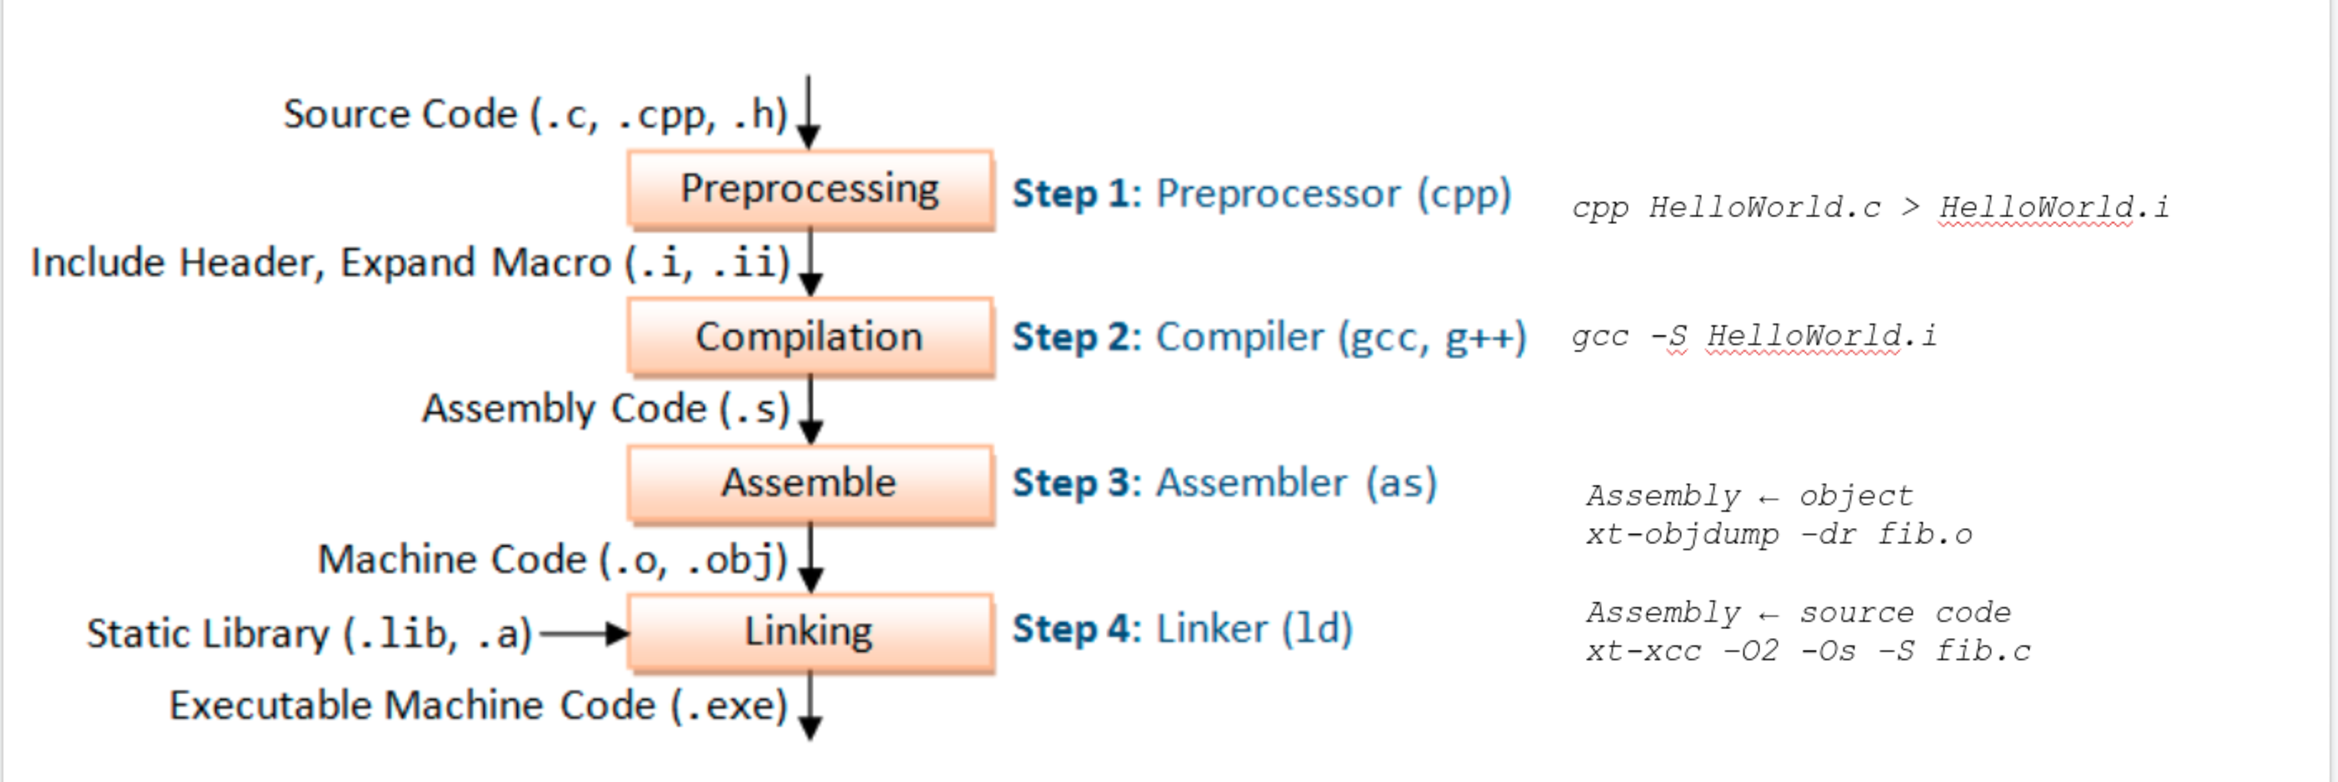
\includegraphics[width=0.5\textwidth]{./build/compilation_steps.pdf}
\end{figure}


\section{Libraries} 
%locations
%LD_LIBRARY
%ldd command

\subsubsection*{Creating Libraries using ar command}%
\label{ssub:creating_libraries_using_ar_command}
ar is an archive tool used to combine objects to create an archive file with .a extension, also known as library.

\href{https://www.thegeekstuff.com/2010/08/ar-command-examples/}{UNIX ar Examples: How To Create, View, Extract, Modify C Archive Files} 

\subsection{pthread} 
% TODO [vikki @22/08/23]: add an examplw with pthread library. %

\subsection{Makefile} 
\href{https://www.gnu.org/software/make/manual/make.html\#toc-Overview-of-make} {GNU make}

Makefile is a utility, which determines automatically which pieces of a large program need to be recompiled, and issues the commands to recompile them.
You can use make with any programming language whose compiler can be run with a shell command. Indeed, make is not limited to programs. You can use it to describe any task where some files must be updated automatically from others whenever the others change.
The make program uses the makefile data base and the last-modification times of the files to decide which of the files need to be updated.
An automation tool for transforming source code into executable  applications 
ar - create, modify, and extract from archives. 

\subsubsection{Getting help}%
\label{ssub:getting_help}
\begin{itemize}
  \item \texttt{man make}
  \item \texttt{make --help}
  \item \href{https://www3.ntu.edu.sg/home/ehchua/programming/cpp/gcc_make.html} { GCC and Make Compiling, Linking and Building C/C++ Applications }
    \item \href{Managing Projects with GNU Make, Third Edition}{https://www.oreilly.com/openbook/make3/book/} 
\end{itemize}



\subsection{bazel} 

